\documentclass[12pt, a4paper, twoside, chapter=TITLE, subsection=TITLE,
section=TITLE, subsubsection=TITLE, english, brazil]{abntex2}

\usepackage[utf8]{inputenc}
\usepackage[brazilian,hyperpageref]{backref}
\usepackage{pacotes}
\usepackage{booktabs}
\usepackage{array}
\usepackage{longtable}
\usepackage{placeins}

\titulo{Classificação do Dataset Iris: Análise Exploratória, PCA e K-NN}
\tituloestrangeiro{Iris Dataset Classification: Exploratory Analysis, PCA and K-NN}
\autor{Bruno Sime Ferreira Nunes -- GRR20190568}
\orientador{Prof. Eduardo Todt}
\data{2026}
\instituicao{
    Universidade Federal do Paraná (UFPR) \par
    Disciplina de Visão Computacional e Percepção
}
\tipotrabalho{Trabalho Acadêmico -- T04}
\local{Curitiba, PR}
\preambulo{Trabalho acadêmico apresentado como requisito de avaliação na disciplina de Visão Computacional e Percepção da Universidade Federal do Paraná.}

\makeatletter
\hypersetup{
    pdftitle={\@title},
    pdfauthor={\@author},
    pdfsubject={\imprimirpreambulo},
    pdfkeywords={Iris}{classificação}{K-NN}{PCA}{aprendizado de máquina},
    pdfcreator={LaTeX with abnTeX2},
    colorlinks=true,
    linkcolor=blue,
    citecolor=blue,
    urlcolor=blue
}
\makeatother

\setlength{\absparsep}{18pt}
\setlength{\parindent}{1.25cm}
\setlength{\parskip}{0pt}
\OnehalfSpacing

\begin{document}
\pretextual
\imprimircapa
\imprimirfolhaderosto[]*
\makeatother\cleardoublepage

\begin{resumo}[Resumo]
Este trabalho apresenta uma análise exploratória e experimentos de classificação no conjunto de dados Iris. Foram calculadas estatísticas descritivas gerais e por espécie, analisadas as relações entre comprimento e largura de sépalas e pétalas e estudada a distribuição conjunta das quatro medidas. A Análise de Componentes Principais mostrou que os dois primeiros componentes preservam 95,81\% da variância total. Para classificação, os dados foram separados de forma estratificada em 80\% para treinamento e 20\% para teste. Um classificador K-Nearest Neighbors, com padronização e seleção de $k$ por validação cruzada, obteve 86,7\% de acurácia no conjunto de teste. Os resultados confirmam que as medidas de pétala são as mais discriminativas e que os erros se concentram entre as espécies \textit{versicolor} e \textit{virginica}.

\vspace{\onelineskip}
\noindent
\textbf{Palavras-chave}: Iris. classificação. K-NN. análise de componentes principais. aprendizado de máquina.
\end{resumo}

\pdfbookmark[0]{\contentsname}{toc}
\tableofcontents*
\cleardoublepage

\textual

\chapter{INTRODUÇÃO}
O conjunto de dados Iris é um dos exemplos clássicos de classificação estatística. Ele contém 150 observações de flores, divididas igualmente entre as espécies \textit{Iris setosa}, \textit{Iris versicolor} e \textit{Iris virginica}. Cada observação possui quatro medidas contínuas, em centímetros: comprimento e largura da sépala e comprimento e largura da pétala. Não há valores ausentes (FISHER, 1936).

O objetivo deste trabalho é caracterizar estatisticamente essas variáveis, examinar a separação visual das espécies, reduzir a dimensionalidade por Análise de Componentes Principais (PCA) e avaliar a classificação com K-Nearest Neighbors (K-NN). O relatório enfatiza a interpretação dos resultados e mantém o conjunto de teste isolado durante a escolha do modelo.

\chapter{MATERIAIS E MÉTODOS}
\section{Conjunto de dados}
Foi utilizada a versão do dataset Iris distribuída com a linguagem R, compatível com os registros corrigidos descritos pelo UCI Machine Learning Repository. O conjunto possui 150 amostras e quatro atributos numéricos. Cada classe contém 50 amostras, portanto a frequência relativa de cada espécie é 33,33\%.

\section{Estatística descritiva}
Foram calculadas média, desvio padrão amostral e moda para cada variável, tanto no conjunto completo quanto separadamente por espécie. Como as medidas são contínuas e registradas com uma casa decimal, a moda foi obtida sobre os valores observados; em caso de empate, todos os valores modais foram mantidos.

\section{Análise exploratória e PCA}
As relações entre comprimento e largura foram avaliadas com diagramas de dispersão e correlação de Pearson, separadamente para sépalas e pétalas. A distribuição conjunta foi inspecionada por uma matriz de dispersão das quatro variáveis.

PCA transforma as variáveis originais correlacionadas em componentes ortogonais ordenados pela variância explicada (JOLLIFFE; CADIMA, 2016). Antes da decomposição, as quatro medidas foram centralizadas e padronizadas, evitando que diferenças de escala ou dispersão dominassem os componentes.

\section{Classificação com K-NN}
A divisão foi estratificada, com semente 42: 120 amostras (80\%) para treinamento e 30 (20\%) para teste, contendo respectivamente 40 e 10 exemplos de cada espécie. Média e desvio usados na padronização foram estimados somente com os dados de treino.

O valor de $k$ foi escolhido por validação cruzada estratificada em cinco partes dentro do conjunto de treinamento. Foram avaliados os valores ímpares de 1 a 15. Somente após essa seleção o modelo foi avaliado no conjunto de teste, preservando a independência da estimativa final.

\chapter{RESULTADOS E DISCUSSÃO}
\section{Estatística descritiva}

\begin{table}[H]
\centering
\caption{Estatísticas descritivas gerais das quatro variáveis.}
\label{tab:geral}
\begin{tabular}{lccc}
\toprule
Variável & Média & Desvio padrão & Moda \\
\midrule
Comprimento da sépala & 5,843 & 0,828 & 5,0 \\
Largura da sépala & 3,057 & 0,436 & 3,0 \\
Comprimento da pétala & 3,758 & 1,765 & 1,4; 1,5 \\
Largura da pétala & 1,199 & 0,762 & 0,2 \\
\bottomrule
\end{tabular}
\end{table}

\begin{table}[H]
\centering
\caption{Estatísticas descritivas por espécie.}
\label{tab:categoria}
\small
\begin{tabular}{llccc}
\toprule
Espécie & Variável & Média & Desvio padrão & Moda \\
\midrule
\textit{setosa} & Comprimento da sépala & 5,006 & 0,352 & 5,0; 5,1 \\
& Largura da sépala & 3,428 & 0,379 & 3,4 \\
& Comprimento da pétala & 1,462 & 0,174 & 1,4; 1,5 \\
& Largura da pétala & 0,246 & 0,105 & 0,2 \\
\midrule
\textit{versicolor} & Comprimento da sépala & 5,936 & 0,516 & 5,5; 5,6; 5,7 \\
& Largura da sépala & 2,770 & 0,314 & 3,0 \\
& Comprimento da pétala & 4,260 & 0,470 & 4,5 \\
& Largura da pétala & 1,326 & 0,198 & 1,3 \\
\midrule
\textit{virginica} & Comprimento da sépala & 6,588 & 0,636 & 6,3 \\
& Largura da sépala & 2,974 & 0,322 & 3,0 \\
& Comprimento da pétala & 5,552 & 0,552 & 5,1 \\
& Largura da pétala & 2,026 & 0,275 & 1,8 \\
\bottomrule
\end{tabular}
\end{table}

As médias indicam um padrão crescente de tamanho de pétala entre \textit{setosa}, \textit{versicolor} e \textit{virginica}. A largura da sépala não segue a mesma ordem: \textit{setosa} apresenta a maior média. Como as classes são perfeitamente balanceadas, a acurácia não é favorecida por uma categoria majoritária.

\section{Relação entre comprimento e largura da sépala}
\begin{figure}[H]
    \centering
    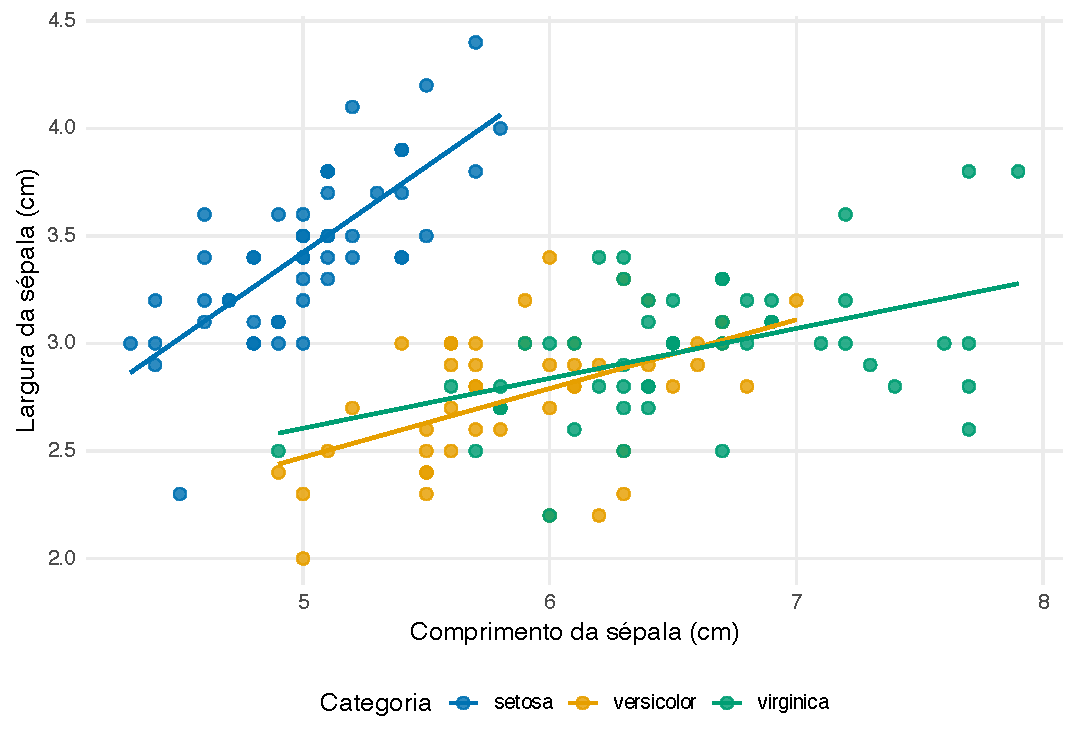
\includegraphics[width=0.88\textwidth]{figuras/sepala.pdf}
    \caption{Comprimento e largura da sépala por espécie.}
    \label{fig:sepala}
\end{figure}

As correlações de Pearson entre comprimento e largura da sépala foram 0,743 para \textit{setosa}, 0,526 para \textit{versicolor} e 0,457 para \textit{virginica}. Embora sejam positivas dentro de cada espécie, existe sobreposição considerável entre \textit{versicolor} e \textit{virginica}. A espécie \textit{setosa} tende a ter sépalas mais curtas e relativamente mais largas.

\section{Relação entre comprimento e largura da pétala}
\begin{figure}[H]
    \centering
    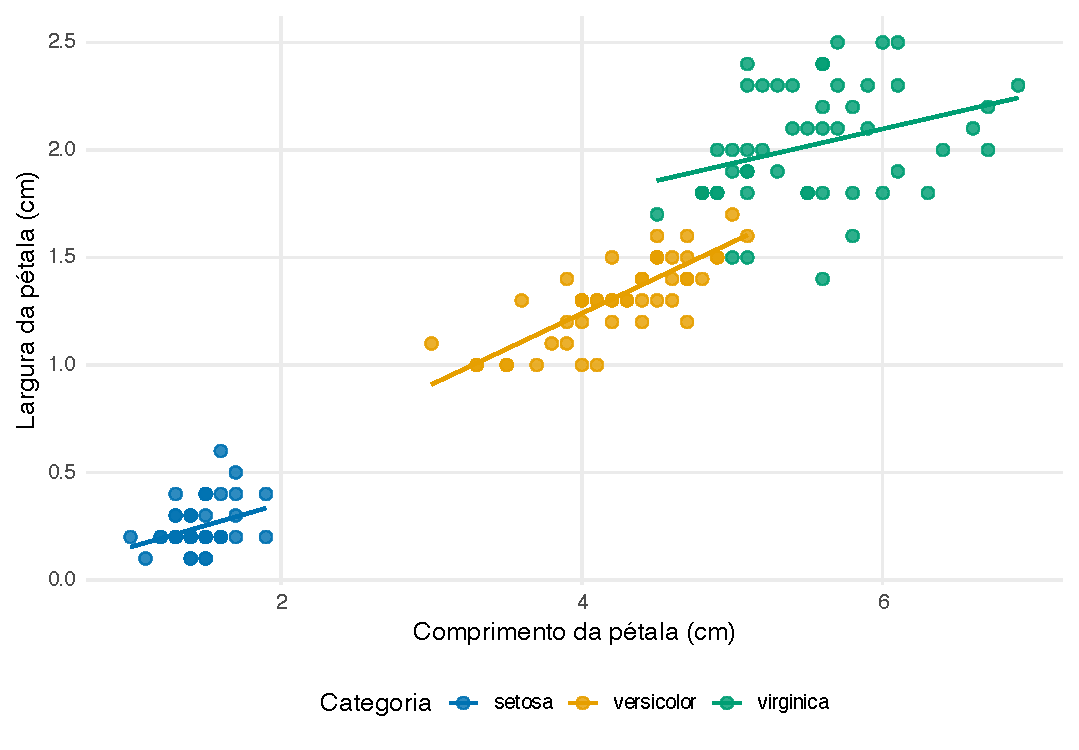
\includegraphics[width=0.88\textwidth]{figuras/petala.pdf}
    \caption{Comprimento e largura da pétala por espécie.}
    \label{fig:petala}
\end{figure}

As correlações entre as duas medidas da pétala foram 0,332 para \textit{setosa}, 0,787 para \textit{versicolor} e 0,322 para \textit{virginica}. A Figura~\ref{fig:petala} mostra uma separação muito mais clara do que a observada nas sépalas: \textit{setosa} forma um grupo isolado, enquanto \textit{versicolor} e \textit{virginica} mantêm apenas uma pequena região de sobreposição.

\section{Distribuição nas quatro dimensões}
\begin{figure}[H]
    \centering
    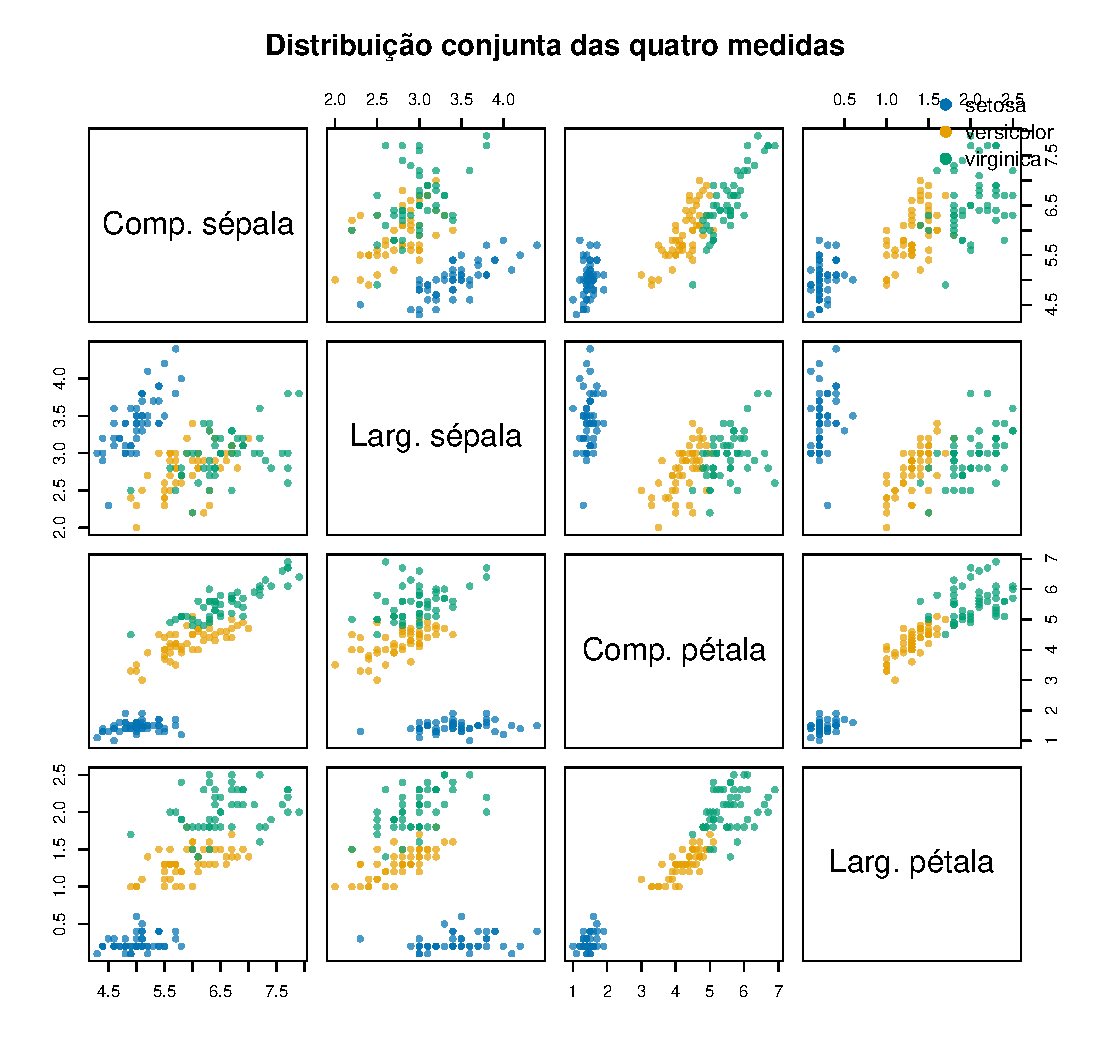
\includegraphics[width=0.91\textwidth]{figuras/pares.pdf}
    \caption{Matriz de dispersão das quatro variáveis do dataset Iris.}
    \label{fig:pares}
\end{figure}

Os pares envolvendo comprimento e largura da pétala são os mais discriminativos. A largura da sépala apresenta a maior sobreposição. A distribuição conjunta confirma que as quatro dimensões contêm informação complementar, mas que grande parte da separação entre as classes está associada às pétalas.

\section{Análise de Componentes Principais}
\begin{table}[H]
\centering
\caption{Variância explicada pelos componentes principais.}
\label{tab:pca}
\begin{tabular}{lcc}
\toprule
Componente & Variância explicada & Variância acumulada \\
\midrule
PC1 & 72,96\% & 72,96\% \\
PC2 & 22,85\% & 95,81\% \\
PC3 & 3,67\% & 99,48\% \\
PC4 & 0,52\% & 100,00\% \\
\bottomrule
\end{tabular}
\end{table}

\begin{figure}[H]
    \centering
    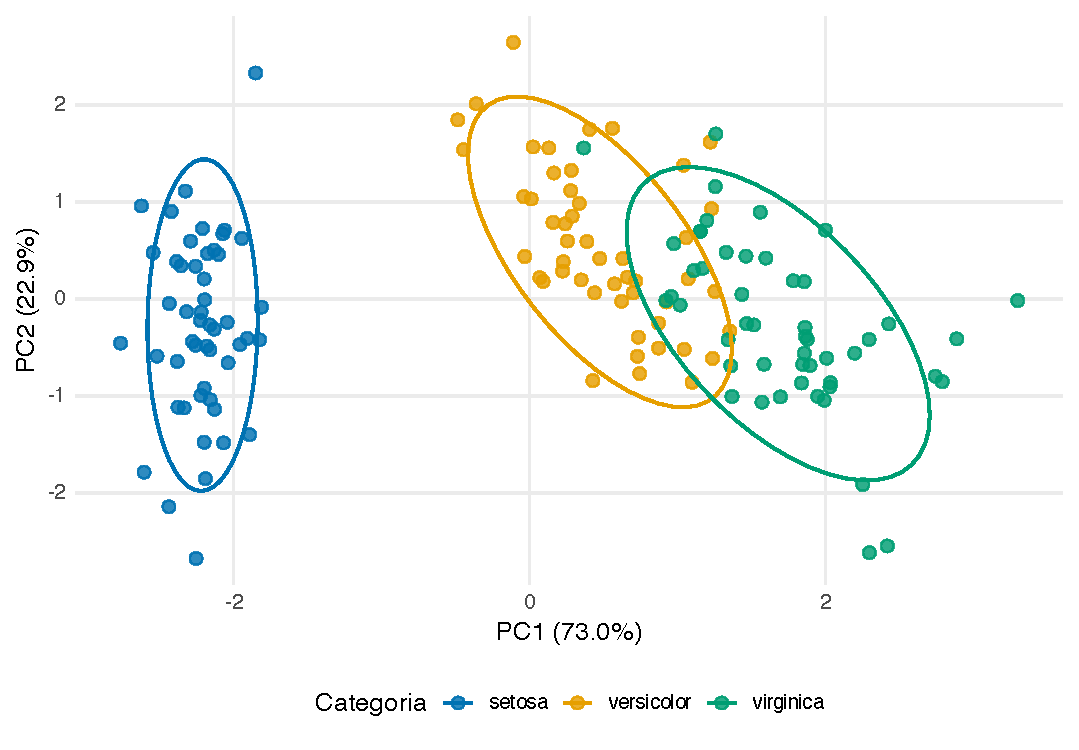
\includegraphics[width=0.88\textwidth]{figuras/pca.pdf}
    \caption{Projeção das amostras nos dois primeiros componentes principais.}
    \label{fig:pca}
\end{figure}

Os dois primeiros componentes preservam 95,81\% da variância total, permitindo representar o conjunto em duas dimensões com pouca perda global. O PC1 recebe contribuições elevadas do comprimento da sépala (0,521), comprimento da pétala (0,580) e largura da pétala (0,565), funcionando aproximadamente como um eixo de tamanho. O PC2 é dominado pela largura da sépala ($-0,923$). A projeção mantém \textit{setosa} claramente separada e evidencia a proximidade entre \textit{versicolor} e \textit{virginica}.

\section{Classificação com K-NN}
\begin{figure}[H]
    \centering
    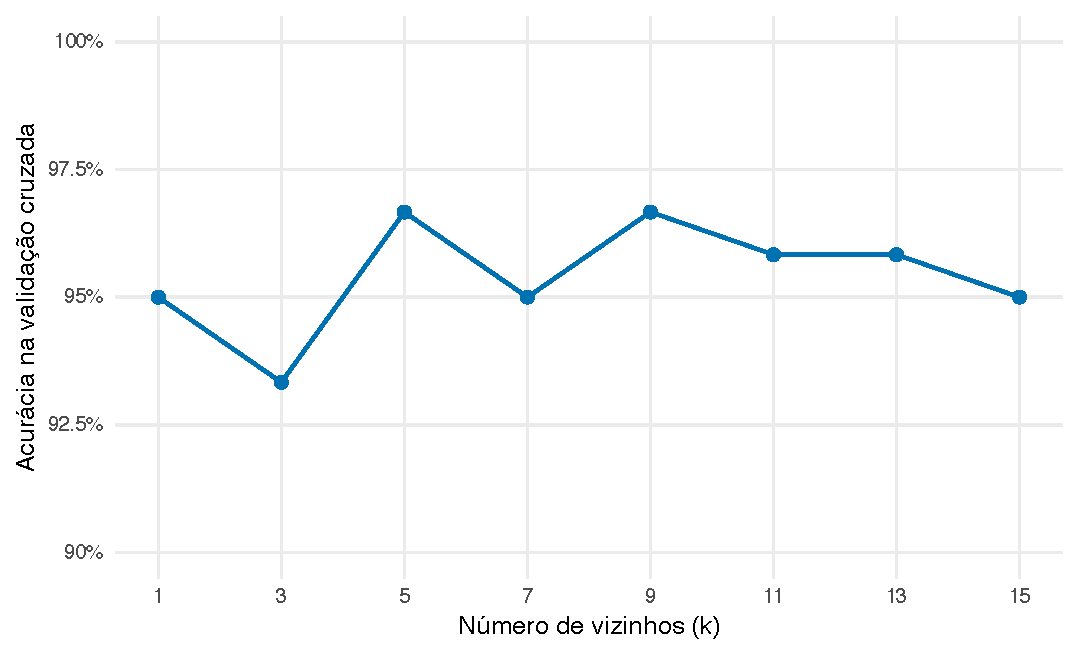
\includegraphics[width=0.86\textwidth]{figuras/knn_cv.pdf}
    \caption{Acurácia da validação cruzada em função do número de vizinhos.}
    \label{fig:knncv}
\end{figure}

Os maiores valores de acurácia média na validação cruzada foram obtidos com $k=5$ e $k=9$, ambos com 96,7\%. Adotou-se $k=5$, o menor valor entre os empatados. No conjunto de teste, a matriz de confusão foi:

\begin{table}[H]
\centering
\caption{Matriz de confusão no conjunto de teste ($n=30$).}
\label{tab:confusao}
\begin{tabular}{lccc}
\toprule
Real / predita & \textit{setosa} & \textit{versicolor} & \textit{virginica} \\
\midrule
\textit{setosa} & 9 & 1 & 0 \\
\textit{versicolor} & 0 & 9 & 1 \\
\textit{virginica} & 0 & 2 & 8 \\
\bottomrule
\end{tabular}
\end{table}

\begin{table}[H]
\centering
\caption{Métricas por espécie no conjunto de teste.}
\label{tab:metricas}
\begin{tabular}{lccc}
\toprule
Espécie & Precisão & Revocação & F1 \\
\midrule
\textit{setosa} & 1,000 & 0,900 & 0,947 \\
\textit{versicolor} & 0,750 & 0,900 & 0,818 \\
\textit{virginica} & 0,889 & 0,800 & 0,842 \\
\bottomrule
\end{tabular}
\end{table}

O classificador acertou 26 das 30 amostras, resultando em 86,7\% de acurácia. Os erros ocorreram sobretudo entre \textit{versicolor} e \textit{virginica}, coerentemente com a sobreposição observada nos gráficos. Houve ainda uma amostra de \textit{setosa} classificada como \textit{versicolor}; devido ao conjunto de teste pequeno, cada erro altera a acurácia em 3,33 pontos percentuais, e o resultado deve ser interpretado como uma estimativa dependente da divisão escolhida.

\chapter{CONCLUSÃO}
O dataset Iris é balanceado e apresenta estrutura favorável à classificação. As dimensões das pétalas são as variáveis que melhor distinguem as espécies, enquanto as medidas de sépala, especialmente sua largura, produzem maior sobreposição. A PCA resumiu as quatro variáveis em dois componentes que preservam 95,81\% da variância e mantêm a organização visual das classes.

Com divisão estratificada de 80\% para treino e 20\% para teste, padronização baseada somente no treino e seleção de $k$ por validação cruzada, o K-NN com cinco vizinhos atingiu 86,7\% de acurácia. Os resultados mostram que a combinação das quatro medidas permite boa separação, mas também confirmam que \textit{versicolor} e \textit{virginica} constituem o principal desafio de classificação.

\postextual
\begin{thebibliography}{99}

\bibitem{uci_iris}
FISHER, R. A. \textbf{Iris} [Dataset]. UCI Machine Learning Repository, 1936. DOI: \url{https://doi.org/10.24432/C56C76}. Acesso em: 18 out. 2026.

\bibitem{jolliffe2016}
JOLLIFFE, I. T.; CADIMA, J. Principal component analysis: a review and recent developments. \textbf{Philosophical Transactions of the Royal Society A}, v. 374, 2016. DOI: \url{https://doi.org/10.1098/rsta.2015.0202}.

\bibitem{cover1967}
COVER, T.; HART, P. Nearest neighbor pattern classification. \textbf{IEEE Transactions on Information Theory}, v. 13, n. 1, p. 21--27, 1967.

\end{thebibliography}
\end{document}
